\chapter{トレースログ可視化ツール TraceLogVisualizer の設計}

\section{開発方針}
TLVの開発目標は,汎用性と拡張性を備えることである.

ここで,汎用性とは,可視化表示したいトレースログの形式を制限しないことであり,可視化表示メカニズムをトレースログの形式に依存させないことによって実現する.
具体的には,標準となるトレースログの形式を定義し,可視化表示メカニズムがこれに依存するようにする.
本論文では以後,この形式を標準形式トレースログと呼称する.ターゲット依存のトレースログを標準形式トレースログに変換することにより,トレースログの形式に依存せずに可視化表示が可能となる.

次に,拡張性とは,トレースログに対する可視化表現をユーザレベルで拡張出来ることを表し,可視化表現,また可視化表現とトレースログの対応を抽象化し,独立して定義できるようにすることで実現する.
具体的には,表示する図形,トレースログと表示する図形の対応をテキスト形式でユーザが定義出来るようにし,それらをプラグインとして動的に組み込ませることを指す.

\section{標準形式トレースログ}

TLVの汎用性は,標準形式トレースログを定義し,これにのみ依存させることで実現することを前節で述べた.

本節では,標準形式トレースログを定義するために行ったトレースログの抽象化と,標準形式トレースログの定義について述べる.

\subsection{トレースログの抽象化}

標準形式トレースログを提案するにあたり,トレースログの抽象化を行った.

はじめに,トレースログを時系列にイベントを記録したものと考えた.
次に,イベントとはイベント発生源の属性の変化,イベント発生源の振る舞いと考えた.
ここで,イベント発生源をリソースと呼称し,固有の識別子をもつものとする.
つまりリソースとは,イベントの発生源であり,名前を持ち,固有の属性をもつものと考えることが出来る.
リソースは型により属性,振る舞いを特徴付けられる.
ここでリソースの型をリソースタイプと呼称する.
属性とはリソースが固有にもつ文字列,数値,真偽値で表されるスカラーデータとし,振る舞いとはリソースの行為であるとする.
振る舞いは任意の数のスカラーデータを引数として受け取ることができる.
リソースタイプとリソースの関係は,オブジェクト指向におけるクラスとオブジェクトの関係に類似しており,属性と振る舞いはメンバ変数とメソッドに類似している.
ただし,振る舞いはリソースのなんらかの行為を表現しており,オブジェクト指向におけるメソッドの,メンバ変数を操作するための関数や手続きを表す概念とは異なる.
主に振る舞いは,属性の変化を伴わないイベントを表現するために用いるものである.
振る舞いの引数は,図形描画の際の条件,あるいは描画材料として用いられることを想定している.

図\ref{fig:resourceTypeSample}と図\ref{fig:resourceSample}に,リソースタイプとリソースを図で表現した例を示す.
さらに,図\ref{fig:resourceTypeSampleByTask}に,RTOS(Real-time operating system)におけるタスクの概念をリソースタイプとして表現した例を,図\ref{fig:resourceSampleByTask}にリソースタイプTaskのリソースの例としてMainTaskを示す.

トレースログの抽象化を以下にまとめる.

\begin{description}
\item[トレースログ] \mbox{} \\
時系列にイベントを記録したもの.
\item[イベント] \mbox{} \\
リソースの属性の値の変化,リソースの振る舞い.
\item[リソース] \mbox{} \\
イベントの発生源.固有の名前,属性をもつ.
\item[リソースタイプ] \mbox{} \\
リソースの型.リソースの属性,振る舞いを特徴付ける.
\item[属性] \mbox{} \\
リソースが固有にもつ情報.文字列,数値,真偽値のいずれかで表現されるスカラーデータで表される.
\item[振る舞い] \mbox{} \\
リソースの行為.主に属性の値の変化を伴わない行為をイベントとして記録するために用いることを想定している.
\end{description}

\begin{figure}[h]
\begin{tabular}{cc}
\begin{minipage}{0.5\hsize}
\begin{center}
\includegraphics[scale=0.5]{img/resourceTypeSample.eps}
\caption{リソースタイプ}
\label{fig:resourceTypeSample}
\end{center}
\end{minipage}
\begin{minipage}{0.5\hsize}
\begin{center}
\includegraphics[scale=0.5]{img/resourceSample.eps}
\caption{リソース}
\label{fig:resourceSample}
\end{center}
\end{minipage}
\end{tabular}
\end{figure}

\begin{figure}[h]
\begin{tabular}{ccc}
\begin{minipage}{0.35\hsize}
\begin{center}
\includegraphics[scale=0.5]{img/resourceTypeSampleByTask.eps}
\caption{タスクをリソースタイプTaskとして表現した例}
\label{fig:resourceTypeSampleByTask}
\end{center}
\end{minipage}
\begin{minipage}{0.25\hsize}
\mbox{}\\
\end{minipage}
\begin{minipage}{0.3\hsize}
\begin{center}
\includegraphics[scale=0.5]{img/resourceSampleByTask.eps}
\caption{リソースタイプTaskのリソースMainTaskの例}
\label{fig:resourceSampleByTask}
\end{center}
\end{minipage}
\end{tabular}
\end{figure}

\clearpage

\subsection{標準形式トレースログの定義}

本小節では,前小節で抽象化したトレースログを標準形式トレースログとして定義する.
標準形式トレースログの定義にはEBNF(Extended Backus–Naur Form)および終端記号として正規表現を用いる.
正規表現はスラッシュ記号(/)で挟むとする.

前小節によればトレースログとは時系列にイベントを記録したものであるので,1つのログには時刻とイベントが含まれるべきである.

\begin{EBNF}
TraceLog = { TraceLogLine };
TraceLogLine = "[",Time,"]",Event,"\n";
Time = /^[0-9a-Z]+$/;
\end{EBNF}

トレースログが記録されたファイルのデータを\verb|TraceLog|とした.
また,\verb|TraceLog|を改行記号で区切った1行を\verb|TraceLogLine|とし,トレースログの単位とした.
\verb|TraceLogLine|は"\verb|[|","\verb|]|"で時刻を囲み,その後ろにイベントを記述するものとする.
時刻は\verb|Time|として定義され,数値とアルファベットで構成される.
アルファベットが含まれるのは,10進数以外の時刻を表現できるようにするためである.
これは,時刻の単位として「秒」以外のもの,たとえば「実行命令数」などを表現出来るように考慮したためである.
この定義から時刻には2進数から36進数までを指定できることがわかる.

前小節にてイベントを「リソースの属性の値の変化,リソースの振る舞い」と抽象化した.
そのため,\verb|Event|を次のように定義した.

\begin{EBNF}
Event = Resource,".",(AttributeChange|BehaviorHappen);
\end{EBNF}

リソースはリソース名による直接指定、あるいは型名と属性条件による条件指定の2通りの指定方法を用意した.

\begin{EBNF}
Resource = ResourceName
         | ResourceTypeName,"(",AttributeCondition,")";
ResourceName = Name;
ResourceTypeName = Name;
Name = /^[0-9a-Z_]+$/;
\end{EBNF}

\verb|AttributeChange|は属性の値の変化を,\verb|BehaviorHappen|は振る舞いを表現している.
これらは,リソースとドット"\verb|.|"でつなげることでそのリソース固有のものであることを示す.
リソースの属性の値の変化と振る舞いは以下のように定義した.

\begin{EBNF}
AttributeChange = AttributeName,"=",Value;
AttributeName = Name;
Value = /^[^"\\]+$/;
BehaviorHappen =  BehaviorName,"(",Arguments,")";
BehaviorName = Name;
Arguments = [{Argument,[","]}];
Argument = /^[^"\\]*$/;
\end{EBNF}

リソースの条件指定の際の\verb|AttributeCondition|は以下のように定義する.

\begin{EBNF}
AttributeCondition = BooleanExpression;
BooleanExpression = Boolean
       |ComparisonExpression
       |BooleanExpression,[{LogicalOperator,BooleanExpression}]
       |"(",BooleanExpression,")";
ComparisonExpression = AttributeName,ComparisonOperator,Value;
Boolean = "true"|"false";
LogicalOperator = "&&"|"||";
ComparisonOperator = "=="|"!="|"<"|">"|"<="|">=";
\end{EBNF}

\subsection{標準形式トレースログの例}

前小節の定義を元に記述した標準形式トレースログの例を以下に示す.
例中のリソースは,図\ref{fig:resourceTypeSampleByTask}と図\ref{fig:resourceSampleByTask}に示したリソースタイプTaskのリソースとする.

\begin{EBNF}
[2403010]MAIN_TASK.leaveSVC(ena_tex,ercd=0)
[4496099]MAIN_TASK.state=RUNNABLE
[4496802]TASK(state==RUNNING).preempt()
[4496802]TASK(state==RUNNING).state=RUNNABLE
[4496802]TASK(id==2).dispatch()
\end{EBNF}

\section{可視化表示メカニズムの抽象化}

前節では,トレースログを抽象化し,標準形式トレースログとして定義した.
TLVの可視化表示メカニズムは,この抽象化にのみ依存するように設計されなければならない.
本節では,可視化表現と可視化表現とトレースログの対応を抽象化する.

\subsection{可視化表現}

TLVにおける可視化表現は,2次元直交座標系における図形の描画とする.
x軸は水平方向に右の方向を正の向きとし,y軸は垂直方向に上の方向を正の向きとする.

\subsubsection{座標系}
図形を定義する座標系をローカル座標系,
図形を時系列にマッピングする際の座標系をワールド座標系,
表示デバイスの座標系をデバイス座標系と呼称する.

ローカル座標系において図形を定義する際は,pixel単位による絶対指定か,ワールド座標系に対する割合を\%で指定する相対指定かのいずれかを用いる.

ワールド座標系のx軸は時間軸となる.
ローカル座標系で定義された図形は,表示する時間の領域にワールド変換される.

図\ref{fig:coordinate}に座標系の例を示す.

\begin{figure}[p]
\begin{center}
\includegraphics[scale=0.75]{img/coordinate.eps}
\caption{座標系}
\label{fig:coordinate}
\end{center}
\end{figure}

\subsubsection{基本単位と図形群}
図形の基本単位は楕円形,多角形,四角形,線分,矢印,扇形,文字列とする.

複数の図形を仮想的にz軸方向に階層的に重ねたものを図形群と呼称し,可視化表現の最小単位とする.
図\ref{fig:shapes}に図形群の例を示す.

\begin{figure}[p]
\begin{center}
\includegraphics[scale=0.75]{img/shapes.eps}
\caption{図形群}
\label{fig:shapes}
\end{center}
\end{figure}

\subsection{可視化表現とイベントの対応}

本小節では,前小節で述べた可視化表現とトレースログのイベントをどのように対応づけるのかを述べる.

\subsubsection{可視化の対象}



\subsubsection{可視化の単位}


\section{可視化方法とトレースログの対応}
